\subsection{Adaptive Query Planning with Composite Sources}
\label{sec:planning}
Theorem~\ref{th:claim-delegation} settles \emph{when} a sub-query may be delegated; we now
turn to \emph{how} an engine uses such delegations. Composite sources are discovered while
the query runs, so the engine must integrate a composite's answers into a plan that is
already executing and already holds intermediate state.


\begin{figure}[t]
  \centering
  \begin{subfigure}[b]{0.37\columnwidth}
    \centering
    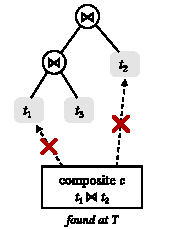
\includegraphics{figures/static-plan.pdf}
    \caption{Static plan: $t_1$ and $t_2$ lie in different subtrees, so $c$ cannot be
      added to the plan.}
    \label{fig:static-plan}
  \end{subfigure}\hfill
  \begin{subfigure}[b]{0.6\columnwidth}
    \centering
    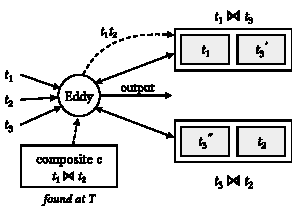
\includegraphics{figures/eddy-join-state.pdf}
    \caption{Eddy: routing history split $t_3$ into $t_3'$ and $t_3''$ across the joins,
      so the $t_1 t_2$ tuples of $c$ probe only $t_3'$.}
    \label{fig:eddy-join-state}
  \end{subfigure}

  \vspace{6pt}
  \begin{subfigure}[b]{0.62\columnwidth}
    \centering
    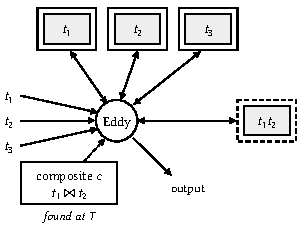
\includegraphics{figures/stem-eddy.pdf}
    \caption{Eddy over SteMs: each pattern has a single SteM, so $c$ becomes a new input
      whose $t_1 t_2$ tuples get a SteM of their own.}
    \label{fig:stem-eddy}
  \end{subfigure}
  \caption{Integrating a composite source $c$, discovered at time $T$ and answering
    $t_1 \bowtie t_2$, into a running plan for $t_1 \bowtie t_2 \bowtie t_3$. Dashed
    elements appear at $T$.}
  \label{fig:integration}
\end{figure}


A static plan fixes its join tree before execution. A composite answering
$t_1 \bowtie t_2$ cannot be used when $t_1$ and $t_2$ lie in different subtrees, since no
operator consumes their joined result (Figure~\ref{fig:static-plan}).

Eddies~\cite{avnur2000eddies} replace the fixed join order by per-tuple routing, but each
join operator keeps the tuples routed to it, so the state of a single pattern is split
across operators by past routing decisions~\cite{deshpande2004lifting}. In
Figure~\ref{fig:eddy-join-state}, $t_3$ is split into $t_3'$ and $t_3''$, and no operator
holds all of $t_3$ for the $t_1 t_2$ tuples of $c$ to probe. Keeping every delegatable
sub-query within one subtree avoids this, but commits the plan in advance to composites
that may never be found, and overlapping candidates such as $t_1 \bowtie t_2$ and
$t_2 \bowtie t_3$ cannot both be kept together. STAIRS~\cite{deshpande2004lifting} lifts
the restriction by migrating state between operators, at the cost of a migration whenever
a new composite is discovered.

Alternatively, an engine can run several plans in
parallel~\cite{tzoumas2010sharing,wei2024rome,justen2024polar}: a default plan beside
plans that join delegatable sub-queries first. These plans are chosen before execution,
whereas the sub-query best delegated to a composite depends on that composite and is known
only once it is found. As different composites may favour overlapping sub-queries, the
required set of plans grows combinatorially and cannot be fixed upfront.

State Modules (SteMs)~\cite{raman2003using} remove the dependence on routing history. A
SteM holds the tuples of a single input and supports \emph{build} and \emph{probe}; a join
becomes two independent half-joins, and intermediate results are not stored. Since each
input has exactly one SteM, its tuples are reachable however earlier tuples were routed.
A composite discovered at runtime simply becomes a new input
(Figure~\ref{fig:stem-eddy}): its $t_1 t_2$ tuples are built into a new SteM and probe the
complete SteM of $t_3$, and $t_3$ tuples arriving later probe the new SteM. No state is
moved and no plan is rebuilt; the price is that intermediate results are recomputed rather
than cached.

\subsubsection{Routing}
\label{sec:routing}

A composite $c$ gives the patterns of its sub-query $B_c \subseteq B$ a second source: a
partial result may take them from the SteM of $c$ or from the base SteMs of $B_c$. The
eddy explores both by routing a copy of the tuple along each, and the copies must stay
apart, so that every pattern of a result is answered by exactly one operator. Each
composite adds such a split, thus composites with overlapping sub-queries should stay separate,
while disjoint composites may occur on the same routing path.
Rather than materialising a plan per combination of composites, we keep a
single eddy and let each tuple carry the constraints of the choices made for it.

\paragraph{Exclusion masks.}
Each operator $o$ is labelled with the patterns it answers, $B_o = \{t\}$ for the SteM of
$t$ and $B_o = B_c$ for a composite, stored as a bitmask over $B$. Every tuple carries a
mask $M$ of the patterns it has answered and a mask $M_{c}$ to indicate if the tuple has
`commited' to a composite during a split.
This constrains the routing to all operators $B_{o}$ that satisfy
\[
    (M \cup M_c) \cap B_o = \emptyset, \forall B_{o} \notin B_{c}
\]

Copies share their route for as long as possible and split lazily: the copy bound for 
$c$ as indicated by $M_{c}$ may pass through SteMs outside $B_c$ before reaching $c$,
and at the split it is stamped $M \gets M \cup B_c$, while the copy that keeps the base route gives up $c$.

This single test keeps the copy away from the base SteMs that $c$ replaces and from every
composite $c'$ with $B_{c'} \cap B_c \neq \emptyset$, so overlapping composites are
mutually exclusive. A composite discovered at runtime adds one operator and its mask; no
existing tuple, SteM or route changes.
The lazy branching allows the router to fully adaptively integrate the composite resource, 
without requiring the composite source to be joined exactly when the split happens in routing.

\begin{figure}[t]
  \centering
  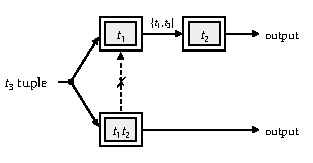
\includegraphics{figures/parallel-routing.pdf}
  \caption{Parallel routing for $t_1 \bowtie t_2 \bowtie t_3$ with a composite $c$ answering
    $t_1 \bowtie t_2$. A $t_3$ tuple splits into a copy that probes the base SteMs and a copy
    bound for $c$, stamped with $B_c$, which bars it from the SteMs that $c$ replaces.}
  \label{fig:parallel-routing}
\end{figure}

\paragraph{Canonical order.}
Copies may still reach the same composites, e.g.\ $c_a$ then $c_b$ and $c_b$ then $c_a$.
To prevent this, at a split the base copy declines every composite offered there, and the
copy bound for $c_j$ declines those with a lower discovery index. Two copies of a split
thus differ on a composite only one of them joins, so each combination of disjoint
composites is produced exactly once.

\todo{Proposition: the eddy emits every solution of $\ev{B}{G^{\alpha}_{\Dd}}$ exactly
once.}

\paragraph{Practical Implementation.}
We follow the table-based routing implementation~\cite{deshpande2004initial} where 
routing is not decided per tuple.  
Instead the tuple is looked up in a
routing table indexed by its mask $M$, and the routing policy reorders this table only every
$k$ tuples.
Adding a composite $c$ turns each entry with $M \cap B_c = \emptyset$ into a list of
alternative routes, the new route holding $c$ and the operators disjoint from both $M$ and
$B_c$.
Whenever a table entry with two \emph{distinct} next operator routes is encountered, the
tuple is pushed to each operator, splitting the join plan.
As masks range over the patterns of $B$ rather than over
operators, a composite adds routes but no states, and the table keeps at most $2^{|B|}$
entries. 

